\documentclass{beamer}
\usepackage{graphicx}
\usepackage{tikz}
\usetikzlibrary{shapes,arrows}
\usepackage{tikz}
\usetheme{default}
%\usecolortheme{seahorse}
\usepackage{default}

  \setbeamertemplate{footline}[page number]
\setbeamertemplate{navigation symbols}{}
\setbeamertemplate{frametitle}[default][center]
\setbeamerfont{frametitle}{shape=\scshape}

\usepackage{color}

{\title{\textsc{Numerical Methods-Lecture V-Newton's Method}}
\author{Trevor Gallen}
\date{}

\begin{document}


\begin{frame}
\titlepage
\end{frame}

\begin{frame}
\frametitle[alignment=center]{Goals}
Aim is to teach numerical methods, give you the tools you need to write down, solve, and estimate models
\bigskip
\begin{enumerate}
\item Interpolation 
\bigskip
\item Numerical derivatives
\bigskip
\item Maximization/minimization 
\bigskip
\begin{itemize}
\item Deterministic, stochastic 
\bigskip
\item Derivative-based, derivative-free
\bigskip
\item Local, global
\bigskip
\end{itemize}
\item Numerical integration/quadrature
\bigskip
\item Bellman equations 
\end{enumerate}
\end{frame}

%\begin{frame}
%\frametitle[alignment=center]{Odds \& Ends}
%\begin{enumerate}
%\item This course runs for 8 weeks, from XXX-XXX.\\
%\item Office hours:  by appointment
%\item E-mail:   XXX %tgallen\@purdue.edu
%\item Grading:  2 homeworks, one ``paper"/model
%\item Course Text:  Judd
%\item Also useful:  Miranda \& Fackler
%\item Various readings
%\end{enumerate}
%\end{frame}

\begin{frame}
\frametitle[alignment=center]{Motivation}
\begin{itemize}
\item We have some function $f(x)$
\bigskip
\item Want to find $x^*$ such that $f(x^*)=0$.  
\bigskip
\item Examples:
\bigskip 
\begin{itemize}
\item Equilibrium conditions: $X^S(p)-X^D(p)=0$
\bigskip
\item Maximization conditions:  $u'(c)-\lambda =0$
\end{itemize}
\end{itemize}
\end{frame}

\begin{frame}
\frametitle[alignment=center]{Newton's Method: Idea}
\begin{enumerate}
\item  Take a linear approximation of function, find slope and intercept
\bigskip
\item Given equation of line, solve for zero
\bigskip
\item Take that new point, repeat.
\end{enumerate}
\end{frame}

\begin{frame}
\frametitle[alignment=center]{Newton's Method Derivation}
\begin{enumerate}
\item  Take Taylor expansion: $f(x)\approx f(x_0) + \left.\frac{\partial f(x)}{\partial x}\right|_{x=x_0}(x-x_0)$
\item  Set equal to zero: $0= f(x_0) + \left.\frac{\partial f(x)}{\partial x}\right|_{x=x_0}(x-x_0)$
\item  Solve for x: $x= x_0-\frac{f(x_0)}{\left.\frac{\partial f(x)}{\partial x}\right|_{x=x_0}} $
\item Call $x$ $x_0$ repeat. 
\end{enumerate}
In other words, the interative procedure:
$$x_{n+1}=x_n-\frac{f(x_n)}{f'(x_n)}$$
\end{frame}

\begin{frame}
\frametitle[alignment=center]{Example: $f(x)=sin(x)$, $x_0=1$}
\begin{enumerate}
\item  $x_1=sin(1)-\frac{sin(1)}{cos(1)}=1-\frac{0.8414}{0.5403}=-0.56$
\bigskip
\item  $x_2=-0.56-\frac{sin(-0.56)}{cos(-0.56)}=-0.56-\frac{0.53}{0.85}=0.07$
\bigskip
\item  $x_3=0.07-\frac{sin(0.07)}{cos(0.07)}=0.07-\frac{0.07}{1}=-1e-4$
\bigskip
\item And so on until $x_i\approx 0$.
\bigskip
\end{enumerate}
Note: I round.
\end{frame}

\begin{frame}
\frametitle[alignment=center]{Do different starting places matter?}
\begin{table}[htdb!]
\centering
\begin{tabular}{lccccc}
\text{Iteration} & \text{Trial 1} & \text{Trial 2} & \text{Trial 3} & \text{Trial 4} & \text{Trial 5}\\
\hline
0 & 1 & 0.5 & 2 & 3.5 & 1.4 \\
1 & -.56 & -0.05 & 4.1 & 3.13 & -4.40 \\
2 & 0.07 & 3e-5 & 2.4 & 3.14 & 1.32 \\
3 & -1e-4 & -1e-14 & 3.2 & 3.14 & 2.64 \\
$\vdots$ & $\vdots$ & $\vdots$ & $\vdots$ & $\vdots$ & $\vdots$ \\
10 & 0 & 0 & 3.14... & $3.14...$ & 3.14... \\
\end{tabular}
\end{table}
A little, and a lot.
\end{frame}

\begin{frame}
\frametitle[alignment=center]{Newton's Method, Graphically-I}
\begin{figure}[htdb!]
\centering
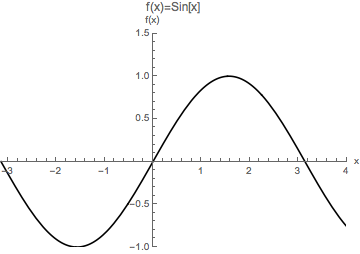
\includegraphics[scale=0.8]{Newton_1.png}
\end{figure}
\end{frame}

\begin{frame}
\frametitle[alignment=center]{Newton's Method, Graphically-II}
\begin{figure}[htdb!]
\centering
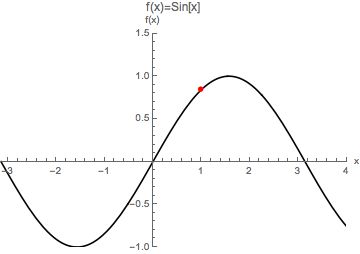
\includegraphics[scale=0.8]{Newton_2.png}
\end{figure}
\end{frame}

\begin{frame}
\frametitle[alignment=center]{Newton's Method, Graphically-III}
\begin{figure}[htdb!]
\centering
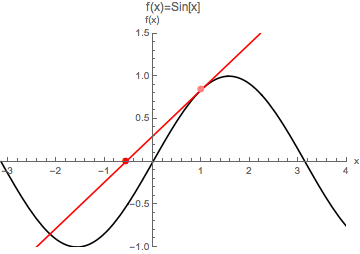
\includegraphics[scale=0.8]{Newton_3.png}
\end{figure}
\end{frame}

\begin{frame}
\frametitle[alignment=center]{Newton's Method, Graphically-IV}
\begin{figure}[htdb!]
\centering
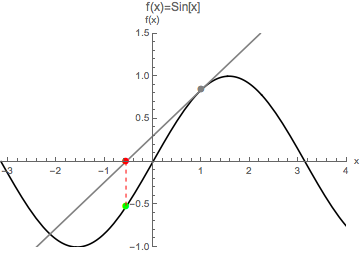
\includegraphics[scale=0.8]{Newton_4.png}
\end{figure}
\end{frame}

\begin{frame}
\frametitle[alignment=center]{Newton's Method, Graphically-V}
\begin{figure}[htdb!]
\centering
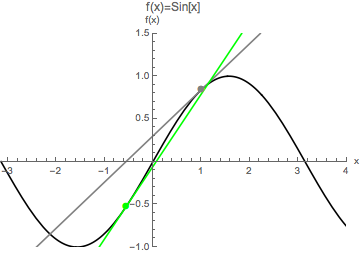
\includegraphics[scale=0.8]{Newton_5.png}
\end{figure}
\end{frame}

\begin{frame}
\frametitle[alignment=center]{Newton's Method, Graphically-VI}
\begin{figure}[htdb!]
\centering
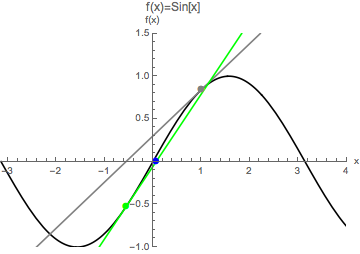
\includegraphics[scale=0.8]{Newton_6.png}
\end{figure}
\end{frame}

\begin{frame}
\frametitle[alignment=center]{Newton's Method, Graphically-VII}
\begin{figure}[htdb!]
\centering
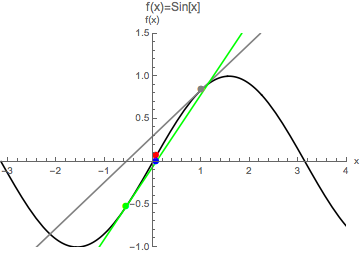
\includegraphics[scale=0.8]{Newton_7.png}
\end{figure}
\end{frame}

\begin{frame}
\frametitle[alignment=center]{Newton's Method, Graphically-VIII}
\begin{figure}[htdb!]
\centering
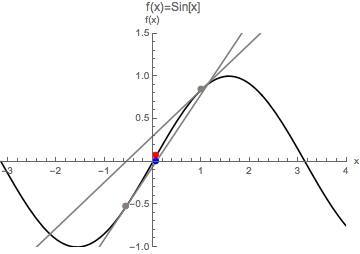
\includegraphics[scale=0.8]{Newton_8.png}
\end{figure}
\end{frame}

\begin{frame}
\frametitle[alignment=center]{Newton's Method, Graphically-IX}
\begin{figure}[htdb!]
\centering
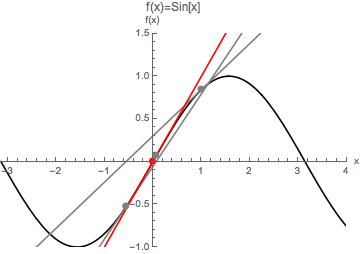
\includegraphics[scale=0.8]{Newton_9.png}
\end{figure}
\end{frame}

\begin{frame}
\frametitle[alignment=center]{Newton's Method, Graphically, New Starting Point}
\begin{figure}[htdb!]
\centering
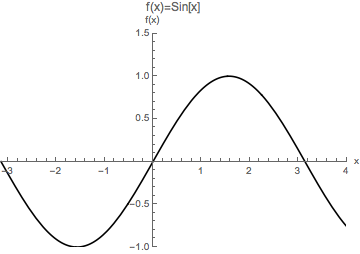
\includegraphics[scale=0.8]{Newton_10.png}
\end{figure}
\end{frame}

\begin{frame}
\frametitle[alignment=center]{Newton's Method, Graphically-XI}
\begin{figure}[htdb!]
\centering
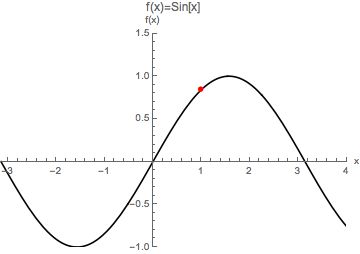
\includegraphics[scale=0.8]{Newton_11.png}
\end{figure}
\end{frame}

\begin{frame}
\frametitle[alignment=center]{Newton's Method, Graphically-XII}
\begin{figure}[htdb!]
\centering
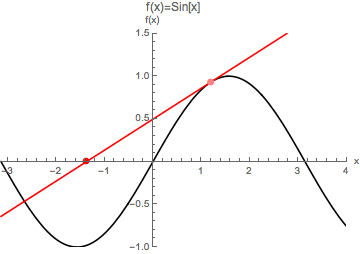
\includegraphics[scale=0.8]{Newton_12.png}
\end{figure}
\end{frame}

\begin{frame}
\frametitle[alignment=center]{Newton's Method, Graphically-XIII}
\begin{figure}[htdb!]
\centering
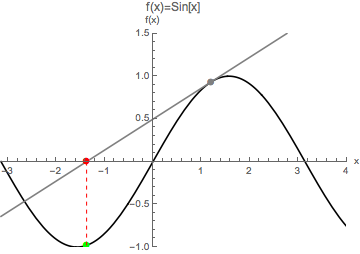
\includegraphics[scale=0.8]{Newton_13.png}
\end{figure}
\end{frame}

\begin{frame}
\frametitle[alignment=center]{Newton's Method, Graphically-XIV}
\begin{figure}[htdb!]
\centering
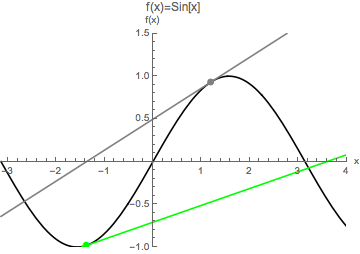
\includegraphics[scale=0.8]{Newton_14.png}
\end{figure}
\end{frame}

\begin{frame}
\frametitle[alignment=center]{Newton's Method, Graphically-XV}
\begin{figure}[htdb!]
\centering
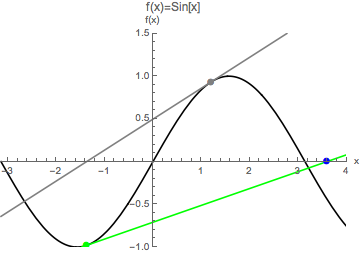
\includegraphics[scale=0.8]{Newton_15.png}
\end{figure}
\end{frame}

\begin{frame}
\frametitle[alignment=center]{Newton's Method, Graphically-XVI}
\begin{figure}[htdb!]
\centering
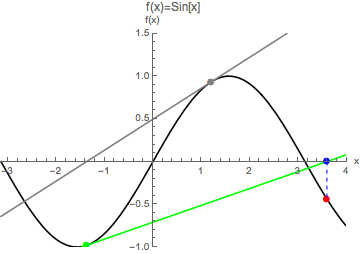
\includegraphics[scale=0.8]{Newton_16.png}
\end{figure}
\end{frame}

\begin{frame}
\frametitle[alignment=center]{Newton's Method, Graphically-XVII}
\begin{figure}[htdb!]
\centering
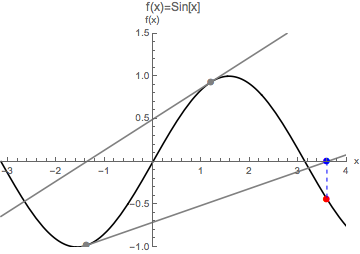
\includegraphics[scale=0.8]{Newton_17.png}
\end{figure}
\end{frame}

\begin{frame}
\frametitle[alignment=center]{Newton's Method, Graphically-XVIII}
\begin{figure}[htdb!]
\centering
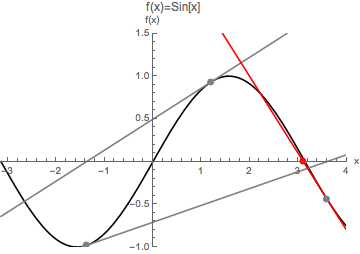
\includegraphics[scale=0.8]{Newton_18.png}
\end{figure}
\end{frame}

\begin{frame}
\frametitle[alignment=center]{Benefits, Costs}
\begin{itemize}
\item Newton's method is quite rapid (locally quadratically convergent)
\bigskip
\item Requires smoothness/derivative
\bigskip
\item Can get trapped at local minima
\bigskip
\item Can be sensitive to starting points
\end{itemize}
\end{frame}

\begin{frame}
\frametitle[alignment=center]{One dimension is easy...how about two?}
Before, scalar equation:
$$f(x)=0$$
Now:
$$\left[\begin{array}{c}f^{[1]}(x_1,x_2) \\ f^{[2]}(x_1,x_2)\end{array}\right]=\left[\begin{array}{c}0 \\ 0\end{array}\right]$$
\end{frame}

\begin{frame}
\frametitle[alignment=center]{Newton's Method: Vector of Equations}
$$\left[\begin{array}{c}f^{[1]}(x_1,x_2) \\ f^{[2]}(x_1,x_2)\end{array}\right]=\left[\begin{array}{c}0 \\ 0\end{array}\right]$$
The Jacobian (matrix of first derivatives):
$$Df = \left[\begin{array}{cc}\frac{\partial f^{[1]}}{\partial x_1} & \frac{\partial f^{[1]}}{\partial x_2} \\\frac{\partial f^{[2]}}{\partial x_1} & \frac{\partial f^{[2]}}{\partial x_2}\end{array}\right]$$
So we can take the multivariate taylor expansion, in matrix form:
$$\left[\begin{array}{c}f^{[1]}(x_1,x_2) \\ f^{[2]}(x_1,x_2)\end{array}\right]\approx \left[\begin{array}{c}f^{[1]}(\overline{x_1},\overline{x_2}) \\ f^{[2]}(\overline{x_1},\overline{x_2})\end{array}\right]+ \left[\begin{array}{cc}\frac{\partial f^{[1]}}{\partial x_1} & \frac{\partial f^{[1]}}{\partial x_2} \\\frac{\partial f^{[2]}}{\partial x_1} & \frac{\partial f^{[2]}}{\partial x_2}\end{array}\right]\left(\left[\begin{array}{c}x_1 \\ x_2\end{array}\right]-\left[\begin{array}{c}\overline{x_1} \\ \overline{x_2}\end{array}\right]\right)$$
\end{frame}

\begin{frame}
\frametitle[alignment=center]{Newton's Method: Vector of Equations}
Set it equal to zero:
$$\left[\begin{array}{c}0 \\ 0\end{array}\right]= \left[\begin{array}{c}f^{[1]}(\overline{x_1},\overline{x_2}) \\ f^{[2]}(\overline{x_1},\overline{x_2})\end{array}\right]+ \left[\begin{array}{cc}\frac{\partial f^{[1]}}{\partial x_1} & \frac{\partial f^{[1]}}{\partial x_2} \\\frac{\partial f^{[2]}}{\partial x_1} & \frac{\partial f^{[2]}}{\partial x_2}\end{array}\right]\left(\left[\begin{array}{c}x_1 \\ x_2\end{array}\right]-\left[\begin{array}{c}\overline{x_1} \\ \overline{x_2}\end{array}\right]\right)$$
Solving for $\left[\begin{array}{c}x_1 \\ x_2\end{array}\right]$ assuming and inverse matrix:
$$\left[\begin{array}{c}x_1 \\ x_2\end{array}\right]=\left[\begin{array}{c}\overline{x_1} \\ \overline{x_2}\end{array}\right]-\left[\begin{array}{cc}\frac{\partial f^{[1]}}{\partial x_1} & \frac{\partial f^{[1]}}{\partial x_2} \\\frac{\partial f^{[2]}}{\partial x_1} & \frac{\partial f^{[2]}}{\partial x_2}\end{array}\right]^{-1}\left[\begin{array}{c}f^{[1]}(\overline{x_1},\overline{x_2}) \\ f^{[2]}(\overline{x_1},\overline{x_2})\end{array}\right]$$
Or, with obvious notation for the vector $X$, $\bar{X}$, $F$, and the jacobian of $F$, $J$:
$$X_{n+1}=\bar{X}_n-J^{-1}F(\bar{X}_n)$$
\end{frame}

\begin{frame}
\frametitle[alignment=center]{Example-I}
$$\left[\begin{array}{c}f^{[1]}(x_1,x_2) \\ f^{[2]}(x_1,x_2)\end{array}\right]=\left[\begin{array}{c}\exp(x_1)-2\exp(x_2) \\ x_1+x_2-3\end{array}\right]$$
So we can write:
$$J(X)=\left[\begin{array}{cc}\exp(x_1) & -2\exp(x_2) \\ 1 & 1\end{array}\right]$$
$$J(X)^{-1}=\frac{1}{\exp(x_1)+2\exp(x_2)}\left[\begin{array}{cc}1 & 2\exp(x_2) \\ -1 & \exp(x_1)\end{array}\right]$$
\end{frame}

\begin{frame}
\frametitle[alignment=center]{Example-II}
Start at $(0,0)$:
$$\left[\begin{array}{c}x_1 \\ x_2\end{array}\right]=\left[\begin{array}{c}0 \\ 0\end{array}\right]-\left[\begin{array}{cc}0.33 & 0.66 \\ -0.33 &  0.66\end{array}\right]^{-1}\left[\begin{array}{c}-1 \\ -3\end{array}\right]=\left[\begin{array}{c}2.33 \\ 0.66\end{array}\right]$$
$$\left[\begin{array}{c}x_1 \\ x_2\end{array}\right]=\left[\begin{array}{c}2.33 \\ 0.66\end{array}\right]-\left[\begin{array}{cc}0.07 & 0.27 \\ -0.07 &  0.72\end{array}\right]^{-1}\left[\begin{array}{c}6.41 \\ 0\end{array}\right]=\left[\begin{array}{c}2.88 \\ 1.11\end{array}\right]$$
And so on until the solution, $x_1=1.84$ and $x_2=1.15$
\end{frame}

\begin{frame}
\frametitle[alignment=center]{Example-II: First equation and zeros}
\begin{figure}[htdb!]
\centering
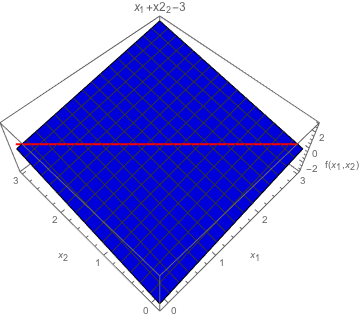
\includegraphics[scale=0.7]{NewtonsMethod_2d_1.png}
\end{figure}

\end{frame}

\begin{frame}
\frametitle[alignment=center]{Example-II: Second equation and zeros}
\begin{figure}[htdb!]
\centering
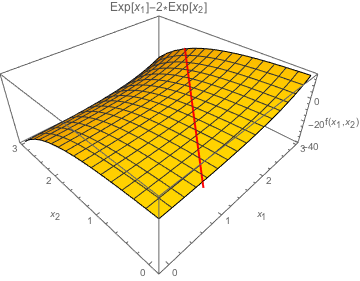
\includegraphics[scale=0.7]{NewtonsMethod_2d_2.png}
\end{figure}
\end{frame}

\begin{frame}
\frametitle[alignment=center]{Example-II: Both Equations and zeros}
\begin{figure}[htdb!]
\centering
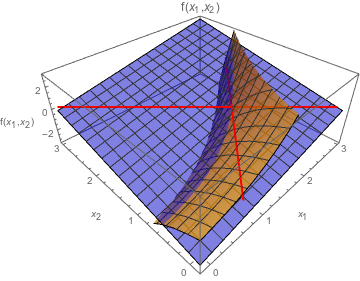
\includegraphics[scale=0.7]{NewtonsMethod_2d_3.png}
\end{figure}
\end{frame}

\begin{frame}
\frametitle[alignment=center]{Example-II: Both Equations and zeros (rotated)}
\begin{figure}[htdb!]
\centering
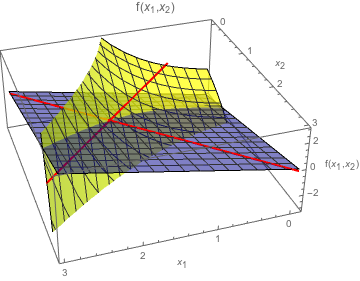
\includegraphics[scale=0.7]{NewtonsMethod_2d_4.png}
\end{figure}
\end{frame}

\begin{frame}
\frametitle[alignment=center]{Equations, approximations, and  zeros}
\begin{figure}[htdb!]
\centering
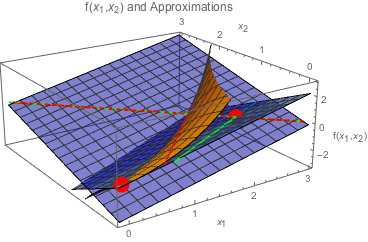
\includegraphics[scale=0.7]{NewtonsMethod_2d_5.png}
\end{figure}
Start at (0,0), take tangent planes, find where planes intersect with zero (green lines), find where lines intersect (new point).  In this case, red and green line are same because linear expansion of linear plane is plane.
\end{frame}

\begin{frame}
\frametitle[alignment=center]{Minimization}
Conceptually, minimization is the same: just find the zeros of the derivative:
$$x_{n+1}=x_n-\frac{f'(x_n)}{f''(x_n)}$$
and:
$$X_{n+1}=X_n-H^{-1}f'(x_n)$$
\end{frame}

\begin{frame}
\frametitle[alignment=center]{Finite Differences}
\begin{itemize}
\item Note that Newton's method assumes you can write derivatives in closed form
\bigskip
\item Much of the time you won't be able to!
\bigskip
\item ``Quasi-Newton" Methods: take finite (forward) differences:
$$\nabla f(x)=\frac{f(x+h)-f(x)}{h}$$
or central differences:
$$\nabla f(x)=\frac{f\left(x+\frac{1}{2}h)-f(x-\frac{1}{2}h\right)}{h}$$
\item This is what Matlab does if you don't give it Jacobian or Hessians
\item Also can approximate Hessians:
\tiny
$$\frac{\partial f'(x,y)}{\partial x\partial y}=\frac{f(x+h,y+h)-f(x+h,y-h)-f(x-h,y+h)+f(x-h,y-h)}{4h^2}$$
\end{itemize}
\end{frame}


\begin{frame}
\frametitle[alignment=center]{Extensions}
\begin{itemize}
\item 80\% of the minimization and solving methods you meet will be derivative-based twists of Newton's Method
\bigskip
\item Halley's Method, Householder Methods: Higher-order derivatives
\bigskip
\item Quasi-Newton Methods: If you can't take $J$, approximate it
\bigskip
\item Secant Method: Newton's Method with finite differences
\bigskip
\item Gauss-Newton: Minimize sum of squared functions
\bigskip
\item Lecture 2 talks about alternatives
\end{itemize}
\end{frame}


\end{document}